\section{Background and Motivation}
\label{sec:background}

In this section we outline the process for defining a UML profile and supporting model editing facilities in Papyrus. 
This process typically involves the manual creation of a number of inter-related models and configuration files.
We highlight labour-intensive and error prone activities involved in the process that motivate the need of automatic generation of those artefacts.

\subsection{UML Profile}
A UML Profile in Papyrus is an EMF model that conforms to the UML Ecore metamodel. 
In order to create a new UML Profile, developers need to create instances of \textit{Stereotype, Property, Association}, etc. to create the elements of their domain specific modeling languages, and their properties and relationships among the elements.

Papyrus offers, among other choices, the mechanism of creating the UML profile using a \textit{Profile Diagram}. 
Users can create UML profile related elements from the palette provided in the UML Profile Diagram editor.
The properties of each element (e.g., data types of properties, multiplicity, navigability, etc.) can then be set using the properties view. 
In a profile, each \textit{Stereotype} needs to extend a UML concept (hereby referred to as \textit{base element} or \textit{meta-element}). 
Users also need to define which \textit{meta-element} their \textit{Stereotype}s extend. 
The users can import meta-elements and add appropriate extension links between their \textit{Stereotypes} and the \textit{meta-elements} by using the tool provided in the palette.
The process of creating the profile can be repetitive and labour-intensive, depending on the size of the profile.
Having created a profile, users can then apply it on a UML model. 
Users typically create instances of UML meta-elements (e.g. UML::Class) and apply their \textit{Stereotype}s defined in their UML profiles. 
For example, if a \textit{Stereotype} extends the ``Class'' meta-element in UML, users can apply it to selected classes in the model. 
In this sense, the users are creating instances of the elements they define in their DSLs. 

One of the limitations of UML Profiles in Papyrus is that links between stereotypes can be instantiated as edges in a diagram only if they extend a \textit{Connector} meta-element (e.g., Association).  
For example, if ``Stereotype A'' refers to ``Stereotype B'' via an ``A\_to\_B'' reference then in order to be able to draw this connection as an edge on the diagram, ``A\_to\_B'' should be created as a separate \textit{Stereotype}. 
These connector \textit{Stereotype}s do not hold any information about the \textit{Stereotype}s that they can connect, so users need to define such restrictions by manually writing OCL constraints to validate at least two things: 1) if the source and target nodes are of the correct type and 2) if the connector is in the correct direction (e.g. the ``A\_to\_B''). 
These constraints can be rather long and need to be manually written and customised for \textit{each} edge \textit{Stereotype}. This can also be a labour-intensive and error-prone process.

\subsection{Distributable Custom Graphical Editor}
With the UML profile created, users can apply it to UML diagrams. 
Users select a UML element (e.g., an instance of UML::Class) and manually apply a \textit{Stereotype} in the UML profile they define. 
A \textit{Stereotype} can only be applied to instances of the meta-elements they extend.
For example, a \textit{Stereotype} that extends the UML::Package meta-element in the profile cannot be applied to an instance of UML::Class. 
This task is obviously labour-intensive and repetitive. 
In addition, the users typically need to remember the meta-element that each \textit{Stereotype} extends in their UML profile. 
%It is even more 
%problematic in scenarios where the profile was created by someone else. In 
%fact, except from using the profile in their local machine, users can 
%distribute it (all the needed information are stored in a file called 
%``model.profile.uml'') so it can be used by others. 

% Although the aforementioned manual creation and use of the profile sometimes covers all the needs of the stakeholders and includes trade-offs they are willing to take, it is usually the case that stakeholders require the definition of custom shapes for the stereotypes and/or a custom palette of stereotypes. The later is important if one thinks that in smaller profiles, users actually need to navigate through tenths of elements available in the default palette, to pick the one that should be used and apply the stereotype. 
To address this recurring concern, Papyrus offers at least three possible options for creating a custom palette which allows users to create UML elements and apply selected \textit{Stereotype}s on them in a single step. 
The first option involves customisation through a user interface where users add elements in the palette for their stereotypes. 
Although this is an easy-to-use approach, it has to be done manually when a new diagram is created. 
In addition, it cannot be shared in case the profile needs to be distributed to collaborators. 
The second option involves the manual definition of a XML-based palette configuration file, which is automatically loaded every time the profile is applied to a diagram. 
This option however, is discouraged by Papyrus as it does not allow the full use of Papyrus functionality.
Furthermore, this option is based on a deprecated framework, and its use is not encouraged. \will{@Thanos, please clarify} \thanos{I believe that this is now clear.}
The third option is to create a UML profile editor, which includes the manual creation of a number of inter-related models and artefacts, including a palette configuration model. 
Although this option provides a whole solution to create a UML profile editor, in the paper we illustrate that this option is a labour-intensive and error prone process.

\begin{figure}[ht]
	\centering
	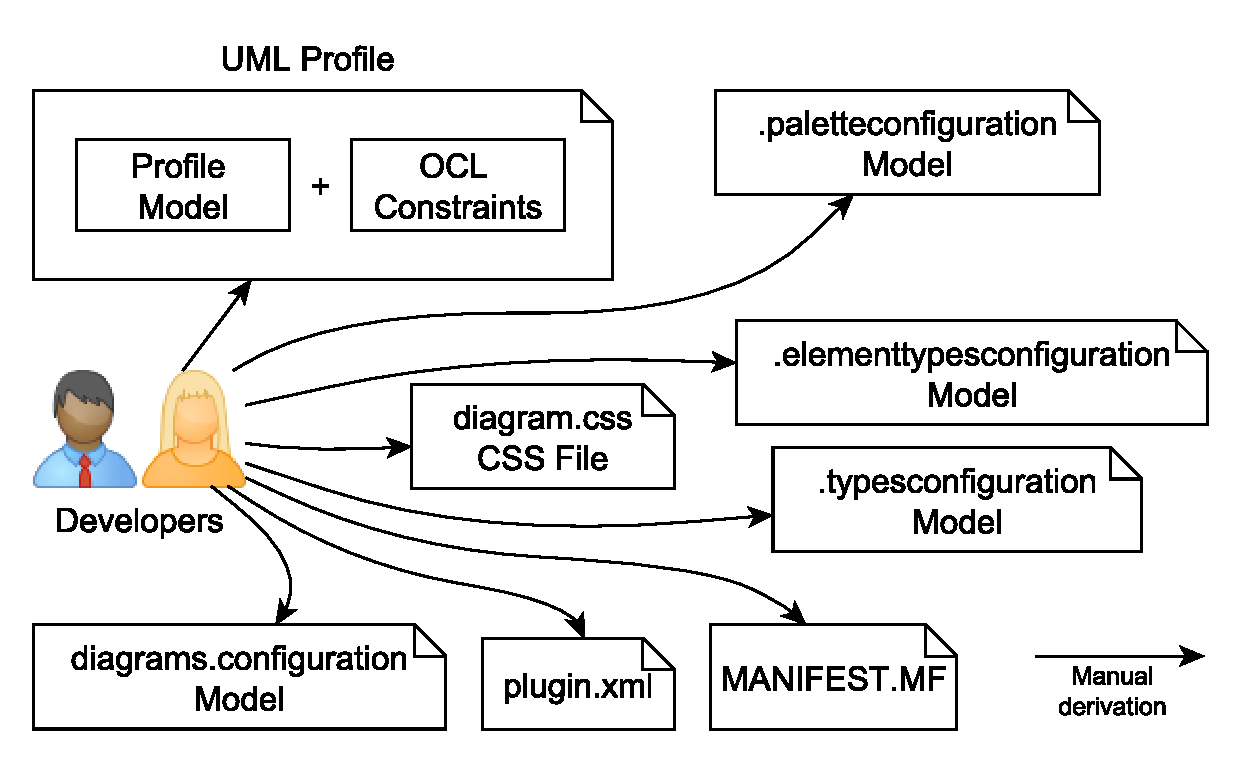
\includegraphics[width=1\textwidth]{diagrams/neededPapyrusFiles.pdf}
	\vspace{-3mm}
	\caption[]{Models/files developers need to write manually to 
		develop a fully functional distributable Papyrus profile editor for Papyrus 2.0.}
	\label{fig:neededPapyrusFiles}
%	\vspace*{-3mm}
\end{figure}

The definition of custom shapes for the instantiated \textit{Stereotype}s is another common requirement. 
In Papyrus, Scalable Vector Graphics (SVG) shapes can be bound to \textit{Stereotype}s during the profile creation process. 
However, to make these shapes visible, users need to set the visibility of the shape of \textit{each} \textit{Stereotype} to true. 
Although this is an acceptable trade-off, the users typically need to hide the default shapes by writing custom style rules in a Cascading Style Sheet (CSS), because that by default the SVG shape bound to a \textit{Stereotype} overlaps with the default shape of the base meta-element.
The CSS can be written once but need to be loaded each time \textit{manually} on every diagram that is created. 

To create a distributable graphical editor that has diagrams tailored for the profile and to avoid all the aforementioned drawbacks, users need to create a number of inter-related models and files, and to implement extension points in an Eclipse plug-in project. 
In our previous work \cite{zolotas2018towards} based on Papyrus 2.0, we identified a number of models that need to be created, which is shown in Figure~\ref{fig:neededPapyrusFiles}. 
To create a working UML profile editor in Papyrus, the users typically need to create a Palette Configuration model, an Element Types Configuration model, a Type Configuration model, a Diagram Configuration model, a CSS and Eclipse plug-in related artefact.
However, in our recent studies we discovered that since Papyrus 3.0, the mechanism for creating UML profile editors had changed, altogether with a number of metamodels. 
Figure~\ref{fig:neededPapyrusFiles_new} shows all the artefacts needed to be created for having a distributable Papyrus UML profile editor for Papyrus 3.0+.
In particular, the Palette Configuration metamodel and the Element Types Configuration metamodel (rendered in blue in Figure~\ref{fig:neededPapyrusFiles_new}) had been changed. 
A new metamodel the Architecture metamodel was introduced (rendered in green in Figure~\ref{fig:neededPapyrusFiles_new}). 
To create a UML profile editor, users also need to create a Creation Command Java class to initialise the UML diagram (rendered in green in Figure~\ref{fig:neededPapyrusFiles_new}). 
This introduces addition complications, because the changes were not properly documented, and there is little documentation on how to create models mentioned in Figure~\ref{fig:neededPapyrusFiles_new} in order to create a working UML profile editor.
In addition, it is also a labour-intensive and error-prone process to migrate editors created based on Papyrus 2.0 to Papyrus 3.0+, for the users typically need to create new Palette Configuration and Element Types Configuration models, as well as the new concepts such as the Architecture model.

\begin{figure}[ht!]
	\centering
	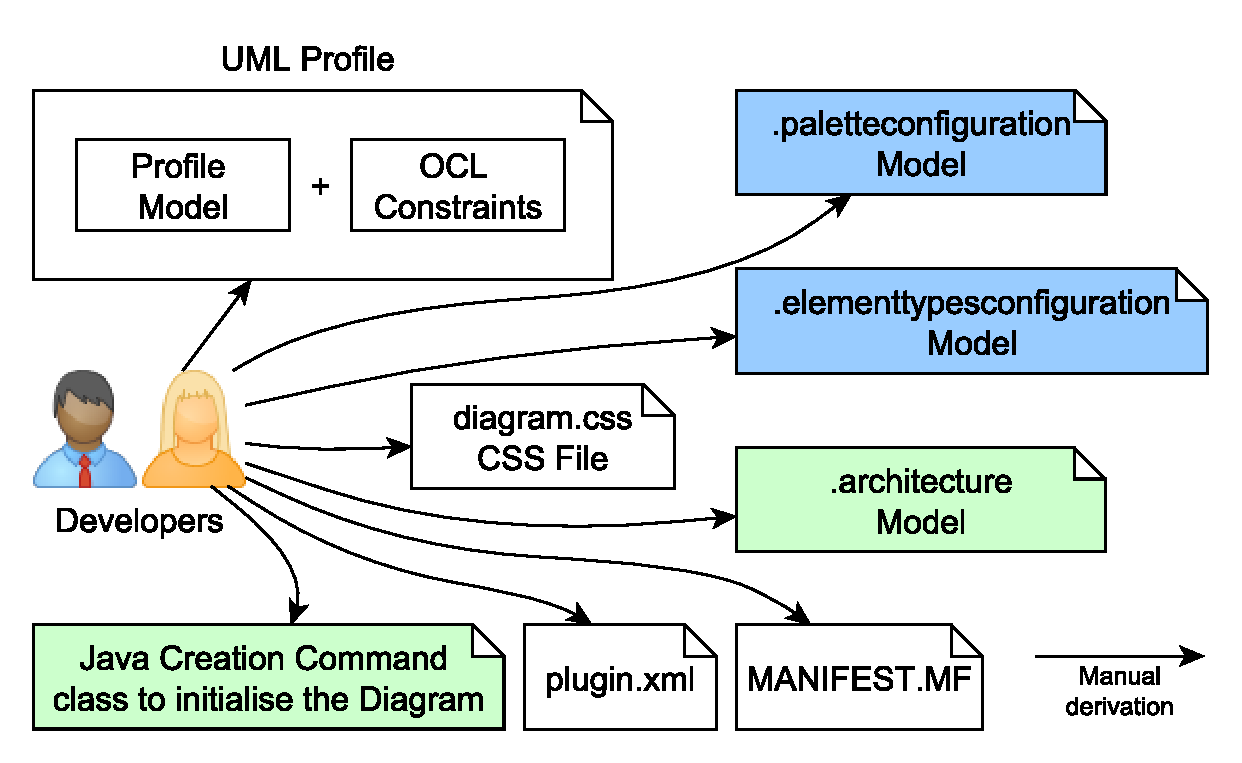
\includegraphics[width=1\textwidth]{diagrams/neededPapyrusFiles_new.pdf}
	\vspace{-3mm}
	\caption[]{Models/files developers need to write manually to 
		develop a fully functional distributable Papyrus profile editor for Papyrus 3.0+.}
	\label{fig:neededPapyrusFiles_new}
%	\vspace*{-3mm}
\end{figure}


UML profile editors created using approaches in Figure~\ref{fig:neededPapyrusFiles} and Figure~\ref{fig:neededPapyrusFiles_new} both have custom palette, with which the users are able to create elements in their DSL (UML meta-elements with \textit{Stereotype}s defined in the UML profile applied automatically to them).
Detailed discussions about the artefacts needed in order to create a UML profile editor are provided in Section~\ref{sec:implementation}.
A few hundred lines of code need to be written while tedious Plug-in creation and repetitive model creation tasks should be done. \will{This is not necessarily the case, the claim is too strong}

This \textit{labour-intensive}, \textit{repetitive} and \textit{error-prone} process could be automated. 
In this paper, we present our tool - Jorvik, which uses a single-source input to automatically generate a UML profile and models/files mentioned above for a UML profile editor. 
This approach is described in Section~\ref{sec:approach} that follows. 
